\newpage
\section{Introduction}
\label{sec:introduction}

% state the learning objective 
The objective of this laboratory assignment is to study a circuit with four elementary meshes and eight nodes. 
This circuit contains an independent voltage source $v_s$, a voltage source dependent from a current $V_d$,
a current source dependent from a voltage $I_b$ and a capacitor $C$. 
Besides this, it has seven resistors, $R_1$, $R_2$, $R_3$, $R_4$, $R_5$, $R_6$ and $R_7$. The circuit can be seen in Figure~\ref{fig:Circuit}.\\
The main goal of our analysis is to compute $v_6$, beginning with its natural solution and then discovering the forced solution. 
We also analysed how $v_6$, $v_s$ and $v_c$ vary with frequency.\\
In Section~\ref{sec:analysis}, a theoretical analysis of the circuit is
presented, using Octave and node method. In Section~\ref{sec:simulation}, the circuit is analysed by
simulation using ngspice. The conclusions of this study are outlined in
Section~\ref{sec:conclusion}. In addiction, the results are compared to the theoretical results obtained in
Section~\ref{sec:analysis}.

\begin{figure}[h!] \centering
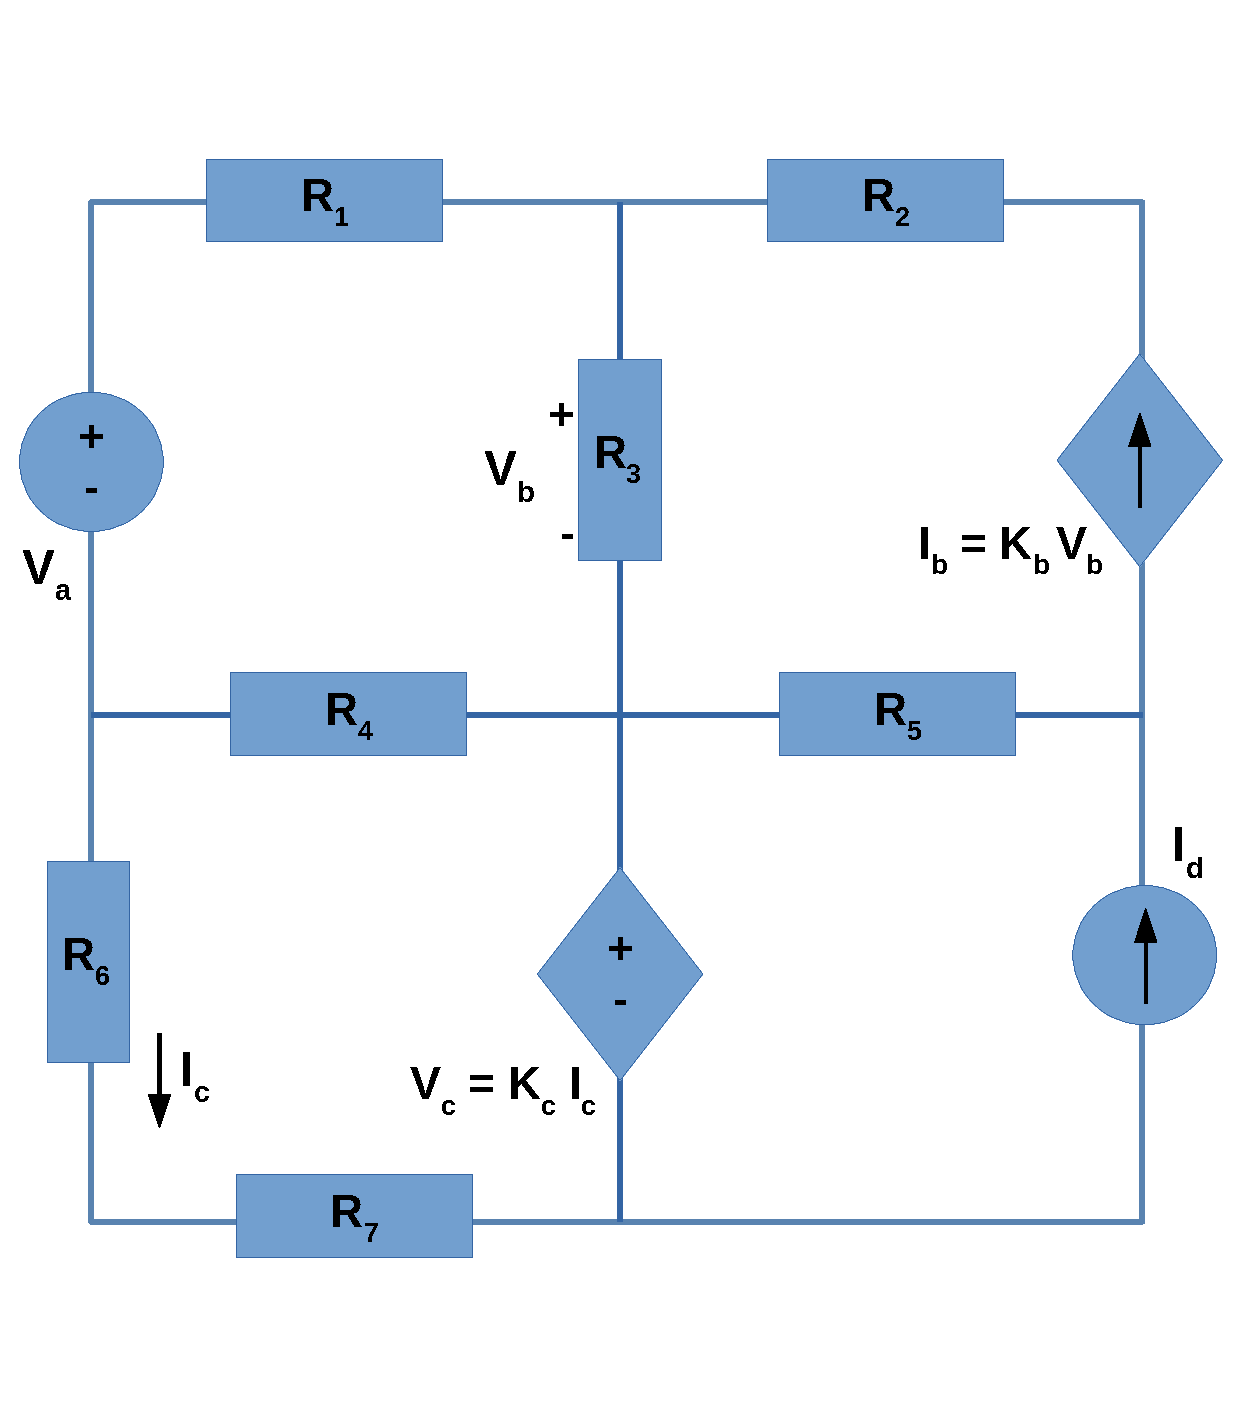
\includegraphics[width=0.6\linewidth]{Circuit.pdf}
\caption{Circuit analysed.}
\label{fig:Circuit}
\end{figure}

